\documentclass[conference]{IEEEtran}

%\usepackage[nocompress]{cite}
\usepackage[english]{babel}
\usepackage{array}
%\usepackage{url}
%\usepackage{amssymb}
%\usepackage{ifthen}
\usepackage{multirow}
\usepackage{csquotes}
\usepackage{fixltx2e}
%\usepackage{enumitem}
%\usepackage{csquotes}
%\usepackage{upquote}
\usepackage{subfigure}
%\setlist{nolistsep}
\usepackage{graphicx}

%common abbreviations
\newcommand{\etal}{{\it et al.}}
\newcommand{\etc}{{\it etc.}}
\newcommand{\ie}{\emph{i.e.}}
\newcommand{\eg}{{\em e.g.}}

%\newboolean{showcomments}
%\setboolean{showcomments}{false}
%
%\ifthenelse{\boolean{showcomments}}
%{ \newcommand{\mynote}[2]{
%    \fbox{\bfseries\sffamily\scriptsize#1}
%    {\small$\blacktriangleright$\textsf{\emph{#2}}$\blacktriangleleft$}}}
%{\newcommand{\mynote}[2]{}}
%
%%Allows to had comments easily with the command \cd{my comment} in the text
%%One command per author (add yours)
%\newcommand{\cd}[1]{\mynote{Corentin}{#1}}
%\newcommand{\ff}[1]{\mynote{Federico}{#1}}
%\newcommand{\todo}[1]{\mynote{TODO}{#1}}

\begin{document}

\title{DC4Cities: Better Usage of the Renewable Energies in Data Centres}

\author{\IEEEauthorblockN{Corentin Dupont}
\IEEEauthorblockA{Create-Net\\
Trento\\
Email: cdupont@create-net.org}
\and
\IEEEauthorblockN{NN 2}
\IEEEauthorblockA{company 2\\
city and code\\
Email: nn@nn.com}
\and
\IEEEauthorblockN{NN 3 etc}
\IEEEauthorblockA{company 3\\
city and code\\
Telephone: xx\\
Fax: xx}}

\maketitle

Energy consumed by data centres in 2010 accounted for between 1.1\% and 1.5\% of the total electricity consumed worldwide~\cite{Koomey2011}, making of data centre energy ma\-nagement an important challenge for researchers.
Contemporary research focused on reducing the overall energy consumption through dedicated Virtual Machine (VM) placement algorithms~\cite{dupont-eenergy12}.
Such algorithms consider the data centre and the workload characteristics to place the VMs among the servers in the most energy-efficient way.
The placement occurs respecting the Service Level Agreements (SLAs) existing between the data centre and its customers.

With the recent adoption of renewable energies to power data centres, the research community enlarges its vision to associate with purely \emph{quantitative} energy consumption reduction, the notion of \emph{quality} of the energy consumed, \ie\ the capacity to rely as much as possible on sustainable power sources~\cite{parasol-sigplan2013}.
Differently from non-renewable energy sources, the availability of renewable energies is very volatile and time dependent: \eg\ solar power is obtainable only during the day, and is subject to variations due to the meteorological conditions.
The goal in this case is to shift the workload of running applications, according to the forecasted availability.

\begin{figure}[ht!]
  \centering
  \subfigure{
     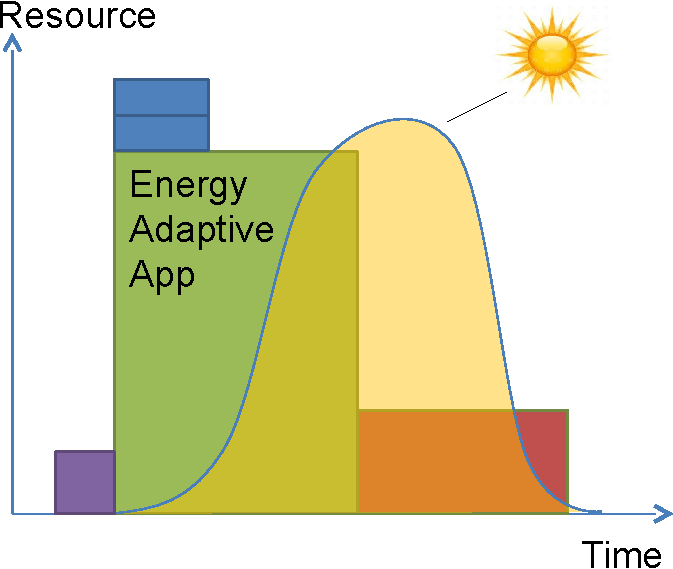
\includegraphics[width=0.42\linewidth]{figs/noadapt}
  }     
  \subfigure{
     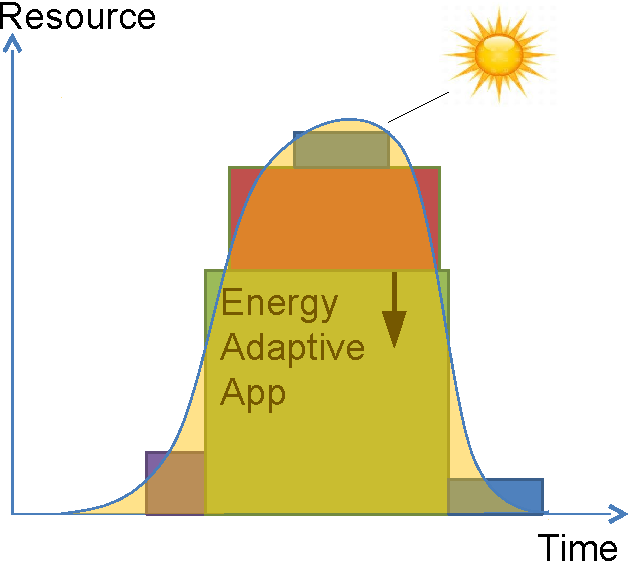
\includegraphics[width=0.40\linewidth]{figs/adapt}
  }     
  \caption{Adapting applications for a better usage of renewable energies}
  \label{fig:adapt}
  \vspace{-1em}
\end{figure}

There is broad agreement that future Smart Cities will depend on IT services that are more and more hosted inside the city.
To maintain a high quality of living inside these cities, the eco-friendliness of data centres relying on local power sources is of high importance.
In this poster, we introduce the initial concepts of DC4Cities, a FP7 project that aims to make data centres more efficient according to the availability of renewable energies, thus better suited for the integration in Smart Cities.
To reach this objective, DC4Cities will propose workload scheduling techniques tightly coupled with energy-adaptive applications that can reconfigure themselves according to power budgets (see Figure~\ref{fig:adapt}).
Combining the two aspects opens up new challenges for the research in the field of energy efficient data centres.

The scenario that we want to support through our research envisions that an external entity located inside a Smart City, called the Energy Management Authority (EMA), will be able to set high-level energy and power objectives for a data centre.
For example, an objective could be: \enquote{at least 80\% of the data centre energy consumption has to be generated from renewable energy sources}.
To translate these high-level objectives into concrete actions performed in the data centre, the platform developed by DC4Cities will need to be informed about the current and future renewable energy availability.
To this end, the DC4Cities platform will receive forecasts regarding the amount of available power and the energy source mix of its electricity inputs.
These forecasts can be either provided directly by the power suppliers or created by algorithms which use environmental and historical data to predict future renewable energy generation.
Having both workload estimations for the different running applications~\cite{Kansal:2008:FEP:1453175.1453180} and the energy forecasts, DC4Cities will be able to assign specific power budgets to the different applications.
The applications, in turn, will have to choose their specific working mode to respect the power budget and the SLAs.

Managing the applications specific workload requires to include in the picture not only the virtual infrastructure layer (IaaS layer) of a data centre, but, as well, the virtual application layer (PaaS layer).
Thus, DC4Cities will extend the VM consolidation techniques to the application layer by: (i) managing elasticity and scalability of multi-tier applications according to their energy footprint (\emph{energy-awareness}); (ii) injecting mechanisms in the single applications to negotiate energy usage according to energy constraints (\emph{energy-adaptiveness}).

The combination of the above techniques will allow:
\begin{itemize}
  \item optimizing \emph{efficient usage of IT equipment}, making sure the workload is concentrated on the minimal amount of hardware (including shutting down unused ones), while preserving the committed SLAs (including GreenSLAs\footnote{GreenSLAs are SLAs that contain flexibility, green KPIs and collaboration options allowing the data centre to operate in a more energy and emission efficient way.}).
  \item ordering, sequencing, shifting of applications in such a way that IT equipment load, and therefore the data centre power consumption, will \emph{adapt to the energy constraints} coming from the data centre operator and from the energy provider.
  \item cooperating with energy-aware applications to make them reconfigure themselves according to power budgets.
  \item automatic splitting and scheduling of system management activities depending on their energy footprint and their level of criticality.
\end{itemize}

\begin{figure}[h]
  \centering
  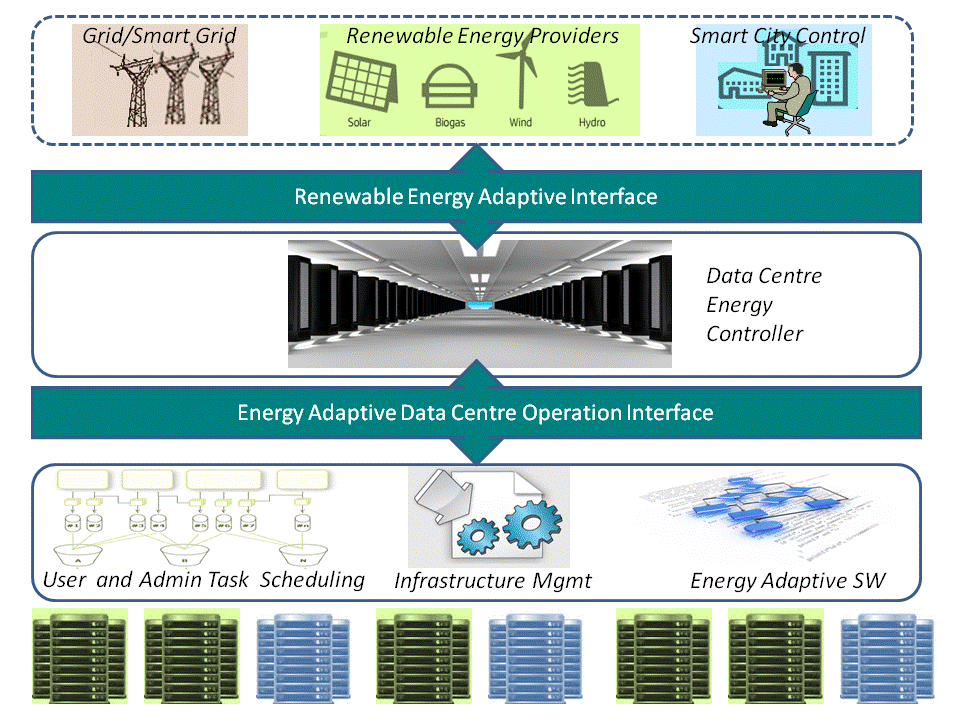
\includegraphics[width=0.99\linewidth]{figs/highlevel}
  \caption{High level architecture}
  \label{fig:architecture}
\end{figure}

The figure~\ref{fig:architecture} provides the high level view of the interactions in the architecture proposed by DC4Cities. The actors can be subdivided in three categories: 
\begin{itemize}
  \item The traditional and renewable energy providers, together with the authorities managing Smart City energy plans, represented in the top row.
  \item The DC4Cities data centre and the data centre energy aware sub-systems, in the lower row.
  \item The DC4Cities Data Centre Energy Controller, represented in the middle of the figure, has a pivotal role: on one side it communicates with the energy providers through the \emph{Renewable Energy Adaptive Interface} (upper interface), and on the other side it communicates with the data centre subsystems through the \emph{Energy Adaptive Data Centre Operation Interface} (lower interface). 
\end{itemize}
The DC4Cities platform will use the upper interface to retrieve informations on renewable energy availability from the respective providers, and will receive energy constraint directives from the EMA and the Smart Grid.
Then, based on the energy availability and constraints, the data centre policies will allow to define, consolidate, optimize and finally enact the energy plans in collaboration with the lower energy adaptive sub-systems. 

New metrics will be developed for the needs of the project, specifically in relation with the energy used in the application domain.
Those metrics will be proposed to standardization bodies.
Finally, the solutions proposed by DC4Cities will be trialled in three different environments: two publicly owned data centres in the city of Barcelona, Spain, and the data centre of the health agency of the province of Trento, Italy.


\section{Acknowledgments}
The authors would like to thank the EU FP7 project DC4Cities (grant agreement number 609304), and the consortium members.

\bibliographystyle{unsrt}
\bibliography{references} 

\end{document}

